
In two dimensions, let \(\vb{x} = (x_1, \dots, x_m)\) and \(\vb{y} = (y_1, \dots, y_m)\).
Then the least squares regression model is given by
\begin{equation}
\label{eqn:ols-model}
f(x) = \frac{\cov(\vb{x},\vb{y})}{\Var(\vb{x})}(x - \overline{\vb{x}}) + \overline{\vb{y}},
\end{equation}
Since \(\vb{x}\) is treated as an input variable and \(\vb{y}\) is treated as an output, this is a type of supervised learning.
In contrast, PCA is an unsupervised learning technique.
PCA organizes the variables in the input space to reveal any patterns in the underlying data.
% \footnote{I think this model would be considered total least squares (TLS) regression since it uses all variables (input and output). Principal component regression (PCR) creates the regression equation using only the input variables.}
If we have input variables \(\vb{x}_1\) and \(\vb{x}_2\), we can use PCA to find a linear pattern among the inputs without trying to predict an output.
First, we find the direction of the largest variance \(\lambda_{\max}\) using the covariance matrix
\[\begin{bmatrix}
\cov(\vb{x}_1, \vb{x}_1) & \cov(\vb{x}_1, \vb{x}_2) \\
\cov(\vb{x}_2, \vb{x}_1) & \cov(\vb{x}_2, \vb{x}_2)
\end{bmatrix} = \begin{bmatrix}
\Var(\vb{x}_1) & \cov(\vb{x}_1, \vb{x}_2) \\
\cov(\vb{x}_1, \vb{x}_2) & \Var(\vb{x}_2)
\end{bmatrix}.\]
In particular,
\[\lambda_{\max} = \frac{1}{2}\left(\Var(\vb{x}) + \Var(\vb{y}) + \sqrt{(\Var(\vb{x}) - \Var(\vb{y}))^2 + 4\cov(\vb{x},\vb{y})^2}\right).\]
Then the PCA regression model becomes
\begin{equation}
\label{eqn:pca-model}
g(x) = \frac{\lambda_{\max} - \Var({\vb{x}_1})}{\cov(\vb{x}_1,\vb{x}_2)}(x - \overline{\vb{x}}_1) + \overline{\vb{x}}_2.
\end{equation}
In this case, the projection residuals are orthogonal to the PCA regression line.
See \Cref{fig:ols-pca}.

\begin{figure}
\centering
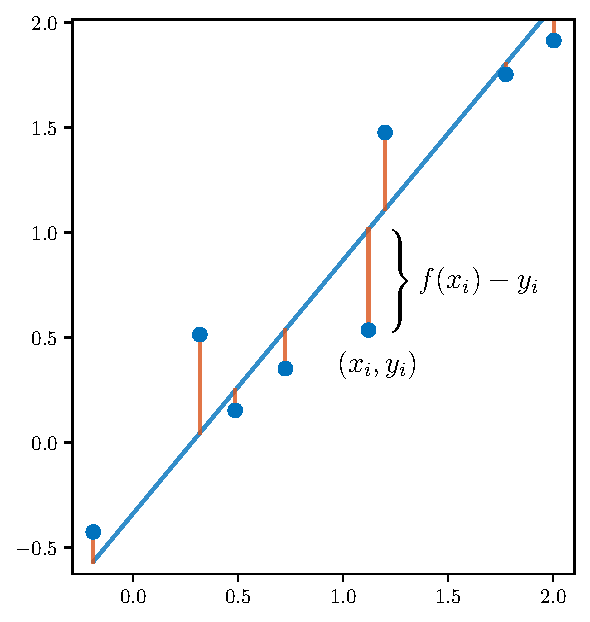
\includegraphics[width=.49\linewidth]{figs/fig-least-squares.pdf}
\hfill
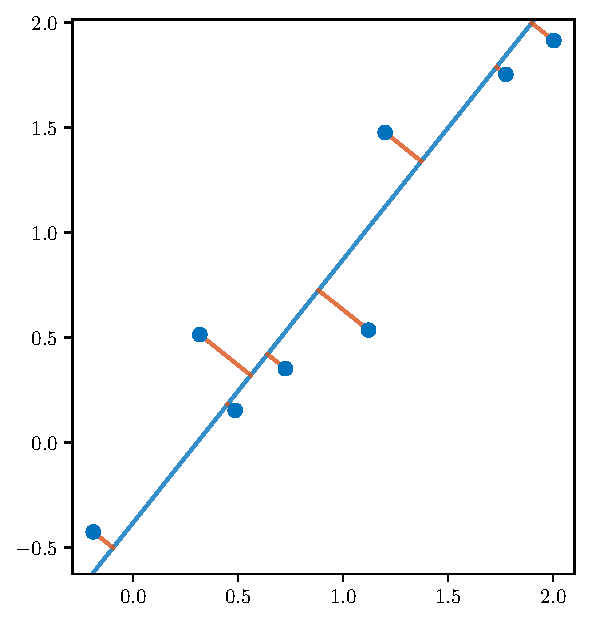
\includegraphics[width=.49\linewidth]{figs/fig-pca-fit.pdf}
\caption{Least squares regression model \(f(x)\) (left) minimizes the sum of squared errors while total least squares, i.e., the PCA model \(g(x)\) (right) minimizes the orthogonal projections.}
\label{fig:ols-pca}
\end{figure}